\chapter{Target Platform}
\label{vehicle_info}

\begin{figure}[H]
	\centering
	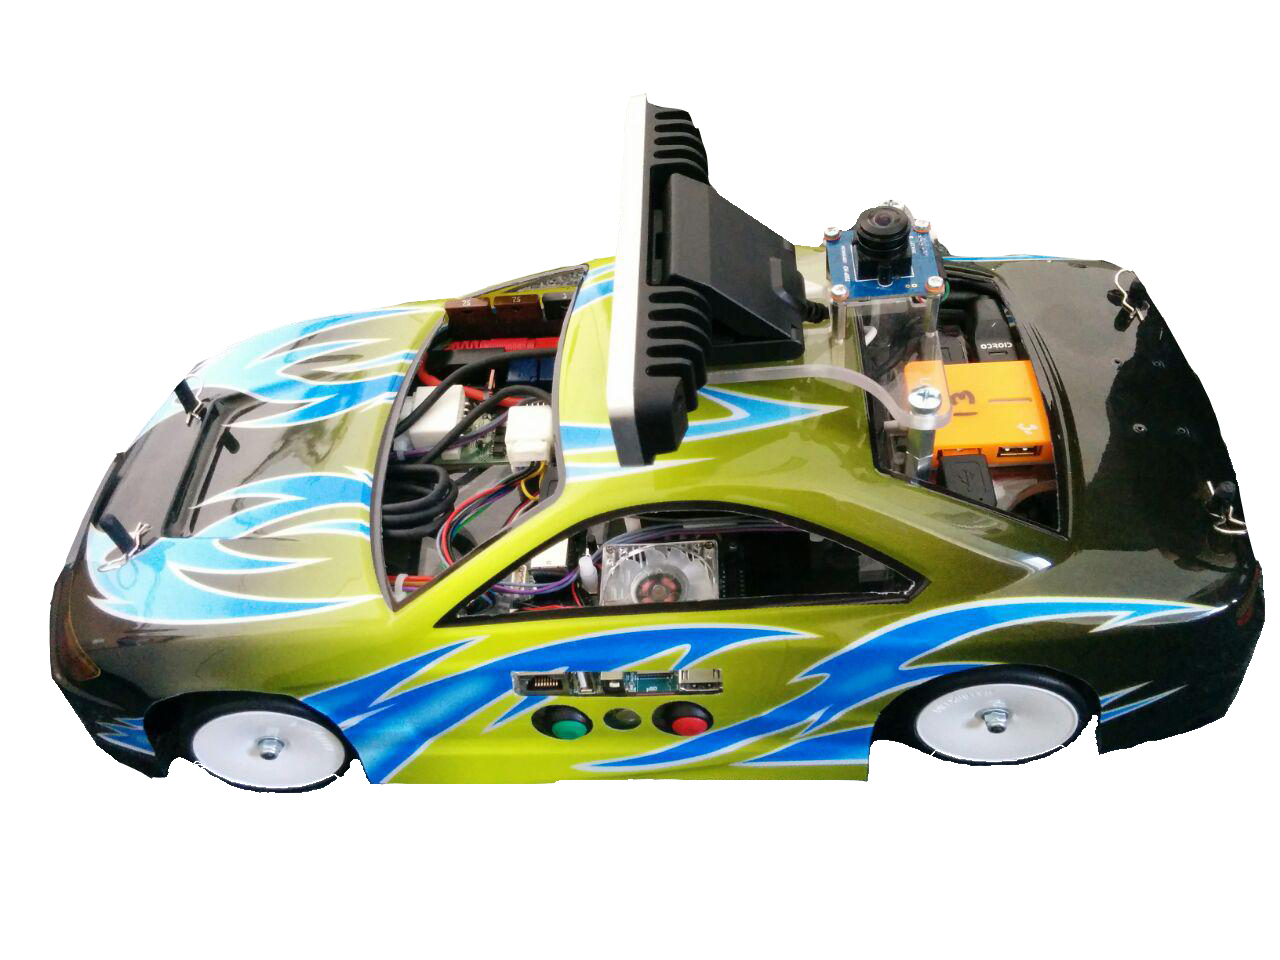
\includegraphics[width=0.6\textwidth]{Images/platform/car.jpg}
	\caption{Model car external view}
	\label{model_car}
\end{figure}

\section{Hardware Components}
The target platform for validating the planner is a 1:10 scale model car (AutoNOMOS Mini V3) as shown in Figure \ref{model_car}, it is developed as an education and research purpose. The car is a modified RC platform,different hardware components used are described in Figure \ref{internalcar}. The main components are a Brushless DC-Servomotor (FAULHABER 2232) to drive and measure speed, servo
motor (HS-645MG) to control the ackerman steering, IMU (MPU6050) to measure the orientation of the car. The 3 modules mentioned are controlled with an Arduino Nano which communicates the data to the main CPU (Odroid XU4). Other important components are a depth camera (intel realsense) for forward vision and perceiving shape of obstacles ahead, 2D-Lidar (RPLidar), WiFi Dongle,  Fish eye Camera for localizing car based on markers on roof. The Figure \ref{moduleconnections} presents connections across different modules present in the car.


\begin{figure}
	\centering
	\includegraphics[width=0.8\textwidth]{Images/platform/car_internals.png}
	\caption{Internal components of Model Car}
	\label{internalcar}
\end{figure}

\begin{figure}
	\centering
	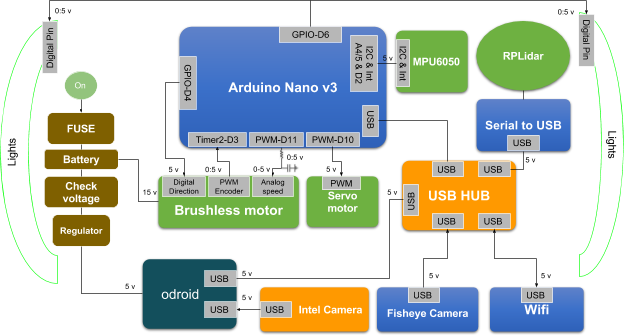
\includegraphics[width=0.8\textwidth]{Images/platform/hardware_Connections.png}
	\caption{Module Connections}
	\label{moduleconnections}
\end{figure}

\section{Software Components}




%\section{Sensors}
%\section{Architecture \& Computational Power}
%\section{Vehicle Control}
%\section{Localisation}
